\documentclass[border=10mm]{standalone}
\usepackage{tikz}
\usepackage{graphicx}  %% for \scalebox
\usetikzlibrary{
  shapes.geometric,
  arrows.meta,
  positioning,
  fit,
  backgrounds,
  decorations.pathreplacing
}

\begin{document}
\scalebox{0.72}{%
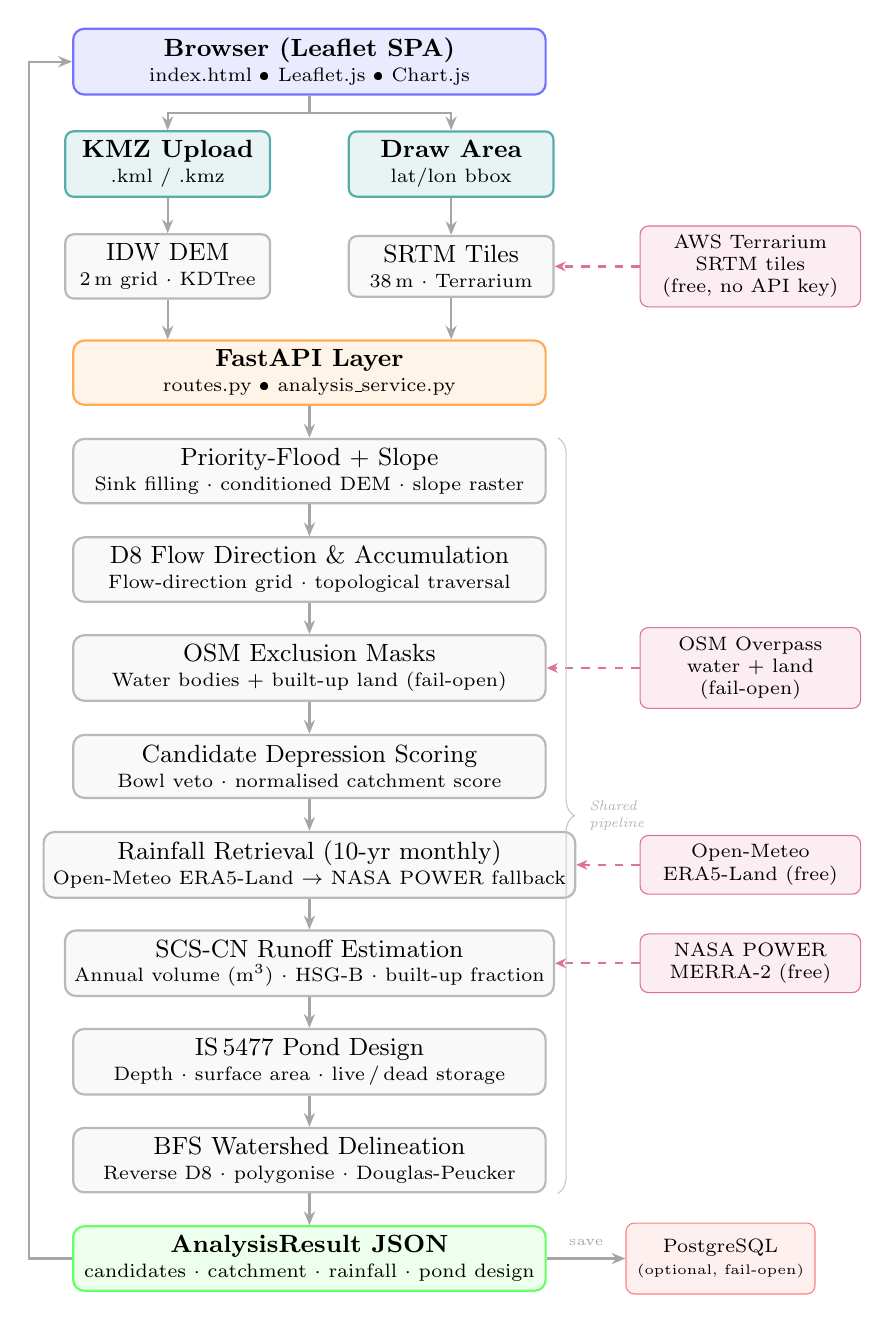
\begin{tikzpicture}[
  font=\small,
  %% ── node styles ────────────────────────────────────────────────────
  %% Wide boxes for full-width pipeline steps
  W/.style  ={rectangle, rounded corners=4pt,
               minimum width=6.0cm, minimum height=0.80cm,
               align=center, thick},
  %% Narrow boxes for side-by-side input/DEM pairs
  N/.style  ={rectangle, rounded corners=3pt,
               minimum width=2.60cm, minimum height=0.75cm,
               align=center, thick},
  %% External API boxes
  EXT/.style={rectangle, rounded corners=3pt,
               draw=purple!55, fill=purple!7,
               minimum width=2.8cm, minimum height=0.65cm,
               align=center, font=\scriptsize},
  %% Arrows
  arr/.style={-{Stealth[length=5pt,width=4pt]}, thick, gray!70},
  ext/.style={-{Stealth[length=4pt,width=3.5pt]}, dashed, thick, purple!55},
]

%% ════════════════════════════════════════════════════════════════════
%% MAIN PIPELINE  (centred at x=0; y steps of -1.25)
%% ════════════════════════════════════════════════════════════════════

%% Row 0 — Browser
\node[W, draw=blue!55, fill=blue!8] (browser) at (0, 0)
  {\textbf{Browser (Leaflet SPA)}\\[-2pt]
   {\scriptsize index.html \textbullet{} Leaflet.js \textbullet{} Chart.js}};

%% Row 1 — Two entry-point labels  (narrow, separated by 3.6 cm)
\node[N, draw=teal!65, fill=teal!9]  (kmz)  at (-1.80, -1.30)
  {\textbf{KMZ Upload}\\[-2pt]{\scriptsize .kml / .kmz}};
\node[N, draw=teal!65, fill=teal!9]  (bbox) at ( 1.80, -1.30)
  {\textbf{Draw Area}\\[-2pt]{\scriptsize lat/lon bbox}};

\draw[arr] (browser.south) -- ++(0,-0.22) -| (kmz.north);
\draw[arr] (browser.south) -- ++(0,-0.22) -| (bbox.north);

%% Row 2 — DEM builders  (narrow; same x as their entry points)
\node[N, draw=gray!55, fill=gray!5] (idw)  at (-1.80, -2.60)
  {IDW DEM\\[-2pt]{\scriptsize 2\,m grid $\cdot$ KDTree}};
\node[N, draw=gray!55, fill=gray!5] (srtm) at ( 1.80, -2.60)
  {SRTM Tiles\\[-2pt]{\scriptsize 38\,m $\cdot$ Terrarium}};

\draw[arr] (kmz)  -- (idw);
\draw[arr] (bbox) -- (srtm);

%% Row 3 — FastAPI  (wide; arrows converge here)
\node[W, draw=orange!65, fill=orange!9] (fastapi) at (0, -3.95)
  {\textbf{FastAPI Layer}\\[-2pt]
   {\scriptsize routes.py \textbullet{} analysis\_service.py}};

%% Angled merge arrows (start at bottom of narrow nodes, end at top corners of FastAPI)
\draw[arr] (idw.south)  -- ++(0,-0.28) -| (fastapi.north -| idw.south);
\draw[arr] (srtm.south) -- ++(0,-0.28) -| (fastapi.north -| srtm.south);

%% Rows 4-11 — Shared pipeline  (wide, all at x=0, step=−1.25)
\node[W, draw=gray!55, fill=gray!5]  (pfill) at (0, -5.20)
  {Priority-Flood + Slope\\[-2pt]
   {\scriptsize Sink filling $\cdot$ conditioned DEM $\cdot$ slope raster}};

\node[W, draw=gray!55, fill=gray!5]  (d8)    at (0, -6.45)
  {D8 Flow Direction \& Accumulation\\[-2pt]
   {\scriptsize Flow-direction grid $\cdot$ topological traversal}};

\node[W, draw=gray!55, fill=gray!5]  (osm)   at (0, -7.70)
  {OSM Exclusion Masks\\[-2pt]
   {\scriptsize Water bodies + built-up land (fail-open)}};

\node[W, draw=gray!55, fill=gray!5]  (cand)  at (0, -8.95)
  {Candidate Depression Scoring\\[-2pt]
   {\scriptsize Bowl veto $\cdot$ normalised catchment score}};

\node[W, draw=gray!55, fill=gray!5]  (rain)  at (0,-10.20)
  {Rainfall Retrieval (10-yr monthly)\\[-2pt]
   {\scriptsize Open-Meteo ERA5-Land $\to$ NASA POWER fallback}};

\node[W, draw=gray!55, fill=gray!5]  (scs)   at (0,-11.45)
  {SCS-CN Runoff Estimation\\[-2pt]
   {\scriptsize Annual volume (m$^3$) $\cdot$ HSG-B $\cdot$ built-up fraction}};

\node[W, draw=gray!55, fill=gray!5]  (is5)   at (0,-12.70)
  {IS\,5477 Pond Design\\[-2pt]
   {\scriptsize Depth $\cdot$ surface area $\cdot$ live\,/\,dead storage}};

\node[W, draw=gray!55, fill=gray!5]  (ws)    at (0,-13.95)
  {BFS Watershed Delineation\\[-2pt]
   {\scriptsize Reverse D8 $\cdot$ polygonise $\cdot$ Douglas-Peucker}};

%% Pipeline arrows (straight down)
\foreach \a/\b in {fastapi/pfill, pfill/d8, d8/osm, osm/cand,
                   cand/rain, rain/scs, scs/is5, is5/ws}
  \draw[arr] (\a) -- (\b);

%% Row 12 — Output
\node[W, draw=green!60, fill=green!7] (result) at (0,-15.20)
  {\textbf{AnalysisResult JSON}\\[-2pt]
   {\scriptsize candidates $\cdot$ catchment $\cdot$ rainfall $\cdot$ pond design}};

\draw[arr] (ws) -- (result);

%% ── PostgreSQL: to the right of result, same row, clear gap ─────────
\node[EXT, draw=red!50, fill=red!6,
      minimum width=2.4cm, minimum height=0.90cm,
      right=1.0cm of result] (db)
  {PostgreSQL\\{\tiny (optional, fail-open)}};

\draw[arr] (result.east) -- node[above,font=\tiny,yshift=1pt]{save} (db.west);

%% ── Return arrow: left spine, clear of all nodes ────────────────────
\draw[arr]
  (result.west)
  -- ++(-0.55, 0)    %% step 5.5 mm left — inside the 10 mm border
  -- ++(0, 15.20)    %% go straight up
  -- (browser.west);

%% ════════════════════════════════════════════════════════════════════
%% EXTERNAL API COLUMN  (x = 5.6, aligned with the step they feed)
%% ════════════════════════════════════════════════════════════════════

\node[EXT] (etile) at (5.6, -2.60)
  {AWS Terrarium\\SRTM tiles\\(free, no API key)};

\node[EXT] (eosm)  at (5.6, -7.70)
  {OSM Overpass\\water + land\\(fail-open)};

\node[EXT] (eom)   at (5.6,-10.20)
  {Open-Meteo\\ERA5-Land (free)};

\node[EXT] (enasa) at (5.6,-11.45)
  {NASA POWER\\MERRA-2 (free)};

%% Dashed arrows from ext column → pipeline nodes
\draw[ext] (etile.west) -- (srtm.east);
\draw[ext] (eosm.west)  -- (osm.east);
\draw[ext] (eom.west)   -- (rain.east);
\draw[ext] (enasa.west) -- (scs.east);

%% ── Shared-pipeline brace  (clear of external nodes) ────────────────
\draw[decorate,
      decoration={brace, amplitude=6pt, raise=4pt},
      gray!45]
  (pfill.north east) -- (ws.south east)
  node[midway, right=12pt, font=\tiny\itshape, text=gray!60, align=left]
  {Shared\\pipeline};

\end{tikzpicture}%
}%
\end{document}
